\section{Research problem}

% Our scope
Formally, we consider the optimal \emph{sequence-to-graph alignment} problem,
the task of finding an optimal base-to-base correspondence between a query
sequence and a (possibly cyclic) walk in the graph. Related alignment problems
have already been formulated as graph shortest path
problems~\cite{jain_complexity_2019}.

%\paragraph{Problem statement}
%\paragraph{Problem domain}

\subsection{Semi-global alignment}

% General: aligning, edit distance
Alignment of reads to a reference genome is an essential and early step in most
bioinformatics pipelines. While linear references have been used traditionally,
an increasing interest is directed towards graph references capable of
representing biological variation~\citep{garrison_variation_2018}.
%
Specifically, a \emph{sequence-to-graph} alignment is a base-to-base
correspondence between a given read and a walk in the graph. As sequencing
errors and biological variation result in inexact read alignments, edit distance
is the most common metric that alignment algorithms optimize in order to find
the most probable read origin in the reference.

% We note that in contrast to linear references, reference graphs capture
% genomic variation and therefore enable more accurate
% alignments~\citep{garrison_variation_2018}.

%\begin{floatingfigure}[l]{0.5\textwidth}
\begin{figure}[t]
    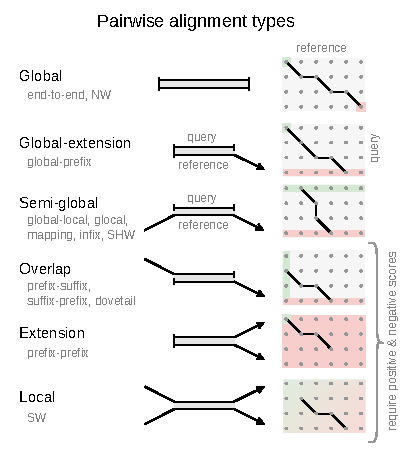
\includegraphics[width=0.5\textwidth]{alignment-types}
	\caption[Alignment types]{Alignment types.}
    \label{fig:alignment-types}
\end{figure}

% paper-trie; seed-and-extend approach to semi-global alignment
\paragraph{Seed-and-Extend}
Since optimal alignment is often intractable, many aligners use heuristics, most
commonly the \emph{seed-and-extend}
paradigm~\cite{altschul_basic_1990,langmead_fast_2012,li_fast_2009}. In this
approach, alignment initiation sites (\emph{seeds}) are determined, which are
then \emph{extended} to form the \emph{alignments} of the query sequence. The
fundamental issue with this approach, however, is that the seeding and extension
phases are mostly decoupled during alignment. Thus, an algorithm with a provably
optimal extension phase may not result in optimal alignments due to the
selection of a suboptimal seed in the first phase. In cases of high sequence
variability, the seeding phase may even fail to find an appropriate seed from
which to extend.

\subsection{Pangenomes and reference graphs}

The shortest path approach naturally fits more complex references than linear.
In fact, any graph reference (incl. cycles) is fine.

% paper-trie; Accounting for variation
%\paragraph{Accounting for Variation}
First attempts to include variation into the reference data structure were made
by augmenting the local alignment method to consider alternative walks during the
extend step~\cite{schneeberger_simultaneous_2009,palmapper}. This approach has
since been extended from the linear reference case to graph references. To
represent non-reference variation of multiple references during the seeding
stage, HISAT2 uses generalized compressed suffix
arrays~\cite{siren_indexing_2014} to index walks in an augmented reference
sequence, forming a local genome graph~\cite{kim_graphbased_2019}.
VG~\cite{garrison_variation_2018} uses a similar
technique~\cite{siren_indexing_2017} to index variation graphs representing a
population of references.

% paper-trie; The benefit from genome graphs
Historically, a single linear reference sequence has been used to represent the
most common variants in a population. While providing a working abstraction for
most cases, rare or sub-population specific variation is especially hard to
model in this setting, creating a reference allele
bias~\cite{stevenson_sources_2013,brandt_mapping_2015}. Consequently, in the
last few years, the field has shifted first towards using sets of reference
sequences, and more recently to graph data structures (so-called {\em genome
graphs}), to represent many genomes or haplotypes
simultaneously~\cite{dilthey_improved_2015,paten_genome_2017,garrison_variation_2018}.

% Sequencing and variant calling
The analysis and understanding of genetic variation encoded in the genome of an
organism lies at the center of computational biology and medicine. Variation is
usually identified through matching sequences obtained from DNA/RNA-sequencing
back to a reference (genome) sequence in the process of \emph{variant calling},
making the alignment task a core problem in sequence bioinformatics.

\subsection{Global alignment}
% paper:seeds
%\subsection{Problem statement: Alignment as shortest path} \label{SEEDsec:task}
%

%\section{Task Description: Alignment to Reference Graphs}
\label{TRIEsec:task}

\paragraph{Dynamic construction}
As the size of the alignment graph is $\Oh(\lvert \RG \rvert \concat \lvert q
\rvert)$, it is expensive to build it fully for every new query.
Therefore, our implementation constructs the alignment graph $\AG$ on-the-fly:
the outgoing edges of a node are only generated on demand and are freed from
memory after alignment.